% !TEX root = Calli.tex

\section{Aufbau}
\label{sec:Kapitel}

Eine einfache Kamera mit USB - Schnittstelle wird mit Hilfe eines Aluprofils 40 cm über dem Spielaufbau positioniert.

%Abbildung Aufbau / Kamera
\begin{figure}[]
    \centering
    \includegraphics[width=5.5cm]{Abbildungen/cover}
    \caption[Anlage]{Anlagenaufbau}
    \label{fig:Anlage}
\end{figure}

Der Spielaufbau entspricht dem original Halli Galli Aufbau mit vier Mitspielern. Um die mittig positionierte Glocke sind die vier Ablagestabel angeordnet. 

%Abbildung Foto, wie die Karten liegen
\begin{figure}[h]
    \centering
    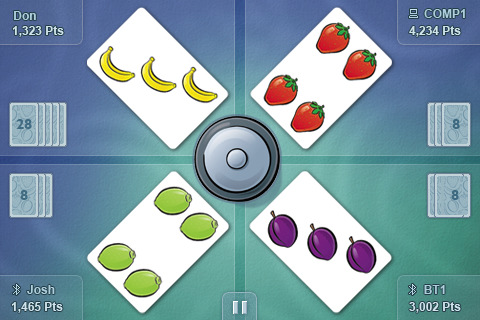
\includegraphics[width=10cm]{Abbildungen/Aufbau}
    \caption[Spielaufbau]{Halli Galli - Spielaufbau mit vier Mitspielern}
    \label{fig:Spielaufbau}
\end{figure}

%Gibt es sonst noch was wichtiges zum Aufbau zu sagen?!?!?
